%\documentclass[a4paper,12pt]{article}
\documentclass[11pt]{article}
\usepackage{graphicx}
\usepackage{amsmath,amsfonts,amsthm,amstext,amssymb}
\usepackage[brazil]{babel}

\usepackage{color}      
\usepackage[utf8]{inputenc}

\usepackage{csquotes}
\usepackage[backend = bibtex,style=numeric-comp,sorting=nyt,date=year,isbn=false,maxnames=10]{biblatex}
\addbibresource{bibliografianova.bib}
%\usepackage[a4paper,top=2cm,bottom=2cm,left=1cm,right=1cm]{geometry}
\usepackage[a4paper, total={6in, 9in}]{geometry}
%\usepackage{setspace} \onehalfspacing
\usepackage{lastpage}
\usepackage{float}
\usepackage{verbatim}
\usepackage{listings}
\usepackage{xcolor}

\newcommand{\R}{\mathbb{R}}
\newcommand{\N}{\mathbb{N}}


\newcommand{\tb}{\mathbf{t}}
\newcommand{\RRR}{\mathbf{R}}
\newcommand{\bsrho}{\boldsymbol{\rho}}
\newcommand{\uu}{\mathbf{u}}
\newcommand{\fm}{\mathbf{f}}
\newcommand{\ds}{\displaystyle}

\usepackage{multirow}
\usepackage[normalem]{ulem}
\useunder{\uline}{\ul}{}
%\usepackage{indentfirst}	
\usepackage{parskip}
\setlength{\parskip}{0.5cm}


\lstset { %
    language=C,
    backgroundcolor=\color{black!3}, % set backgroundcolor
    keywordstyle=\color{black}\bfseries,
    basicstyle=\footnotesize,% basic font setting
}



\begin{document}
\begin{titlepage}
   \begin{center}
       \vspace*{1cm}
 
       \Large
       \textbf{Relatório Final de Iniciação Científica}\\
       Métodos de Otimização aplicados a redes neurais para \\ detecção de anomalias em transações com cartão de crédito
 	   
 	   \normalsize
       \vspace{5.5cm}
        \textbf{Bolsista:} Frederico José Ribeiro Pelogia
        
       \vspace{0.5cm}
        \textbf{Orientador:} Prof. Dr. Luís Felipe Bueno
 
       \vspace{0.5cm}
 
       \textbf{Número do Projeto FAPESP:} 2019/13420-4\\
       
      \vspace{0.5cm}
      
		\textbf{Período de vigência}: 01/09/2019 a 31/08/2020    
      
      \vspace{0.5cm}
		\textbf{Período abordado pelo relatório:} 10/02/2020 a 31/08/2020
 
       \vfill

 
 
       Departamento de Ciência e Tecnologia\\
       Universidade Federal de São Paulo\\
       Julho de 2020
       %-- de -------- de 2020
 
   \end{center}
\end{titlepage}

\section*{Resumo do projeto}
 Neste projeto pretende-se estudar métodos de otimização, em especial algoritmos estocásticos,
aplicados ao treinamento de redes neurais. Em um trabalho\cite{bmLS} recente proposto por E. G. Birgin, L. F. Bueno e
J. M. Martínez, \textit{``On the complexity of solving feasibility problems with regularized models"} , foi apresentado um algoritmo
de primeira ordem com bons resultados de complexidade para problemas de quadrados mínimos.
Um dos principais pontos da pesquisa deste projeto será desenvolver uma versão estocástica desse
algoritmo. Serão analisados os desempenhos dos algoritmos estudados quando aplicados à detecção
de fraudes em operações de cartão de crédito utilizando a base de dados Credit Card Fraud Detection
do Kaggle.

\section*{Resumo das realizações do período}
Este relatório aborda as realizações do período de 10/02/2020 a 31/08/2020. Neste intervalo de tempo, as seguintes atividades foram concluídas:

\begin{itemize}
\item Estudo dos artigos \cite{fraudeItalia1} e \cite{fraudeItalia2}.
\item Experimentar a aplicação dos algoritmos implementados em Python, sem utilização de bibliotecas prontas de \textit{machine learning}, à base de dados Credit Card Fraud Detection.

\item Estudo do método de Levenberg–Marquardt, com base em \cite{TCCKleber}.
\item Estudo teórico de \cite{bmLS}. 
\item Testes associados a \cite{bmLS}.
\end{itemize}

\noindent
Como planejávamos, foi submetido um resumo e um \textbf{vídeo-poster} para apresentação no Congresso Acadêmico UNIFESP 2020, que ocorreu virtualmente, dos dias 13 a 17 de julho.\\

\noindent
Além disso, participamos do desenvolvimento da \textit{Ferramenta de apoio ao planejamento de salas de aula pós pandemia de Covid-19}, que é um site com objetivo de otimizar as posições das carteiras nas salas de aulas de acordo com as medidas de distanciamento propostas pelas autoridades sanitárias. Esse projeto foi desenvolvido com pesquisadores da Instituições Unifesp, UEM e IFSP. Assim, houve contato com técnicas de empacotamento, otimização com restrições e a utilização do software ALGENCAN, do projeto TANGO\cite{TANGO}. É interessante, também, apontar que uma das formulações presentes no projeto envolve um problema de quadrados mínimos. Esse foi um dos fatores principais para o acompanhamento do projeto por parte do bolsista.
\newpage
\section{Estudo dos artigos \cite{fraudeItalia1} e \cite{fraudeItalia2}}
O artigo \cite{fraudeItalia1} aplica redes neurais artificiais ao problema de identificar os determinantes das despesas das unidades locais de saúde da Itália, chamadas de \textbf{LHUs} (Local Health Units). Segundo o mesmo, a utilização das redes neurais é vantajosa pois detecta o que são chamadas de dependências difusas, considerando variáveis que não são completamente captadas por dependências funcionais. A ideia é compreender as similaridades nos dados orçamentarios de saúde em diferentes localidades na Itália.\\

\noindent
O artigo \cite{fraudeItalia2} tem intuito de identificar, dentre os dados de LHUs italianas, sinais de ineficiência e mal gerenciamento dos gastos. Ele investiga a aplicação de um tipo específico de redes neurais, chamado de \textbf{AWIT}\cite{AWIT}(Artificial Neural Networks What-If Theory ) e testa a utilização de uma região italiana como referência para tirar conclusões sobre dados de outras regiões, obtendo  resultados favoráveis. O artigo também afirma que , como os dados orçamentários do sistema de saúde italiano são padronizados e bem detalhados, a aplicação de redes neurais é promissora para esse tipo de identificação.

Em uma apresentação do grupo \textbf{Semeion}\cite{SEMEION}, são comparadas diversas técnicas para detectar fraudes em dados de seguros de saúde na Itália. Os testes com as redes \textbf{AWIT} foram realizados utilizando o \textbf{Semeion Software \#68} e notou-se que essa técnica se destacou em detectar seguros de saúde anômalos baseando-se no número de apólices de seguro direcionadas a certas empresas.


\section{Aplicação dos algoritmos implementados ao problema de deteção de fraudes}
No primeiro semestre de desenvolvimento do projeto, foram estudados e implementados os 9 métodos de otimização a seguir:
\begin{itemize}
\item Método do Gradiente (\textit{Gradient Descent}).
\item Método do Gradiente Estocástico (\textit{SGD}).
\item Método do Gradiente Estocástico com Redução de Variância (\textit{SVRG}).
\item Averaged Stochastic Gradient Descent (\textit{SAG} e \textit{SAGA}).
\item Método do Gradiente com Passo Adaptativo (\textit{Adagrad}).
\item Método \textit{RMSProp}.
\item Métodos com momento de Polyak: foram feitas implementações com o \textit{SGD} e \textit{SVRG}.
\item Métodos com momento de Nesterov: foram feitas implementações com o \textit{SGD} e \textit{SVRG}.
\item Método \textit{Adam}.
\end{itemize}
No Relatório Científico de Progresso, que foi enviado à FAPESP, a ideia de cada um deles foi explicada e foram apresentados 2 tipos de resultado. O primeiro tipo foi uma comparação dos métodos \textbf{implementados} aplicados a um problema de quadrados mínimos simples. O segundo tipo foi a aplicação de alguns dos métodos ao problema de detecção das fraudes do \textit{dataset} de interesse, mas utilizando implementações prontas através da biblioteca Keras\cite{KERAS}. O próximo passo, assim, foi tentar adaptar as versões implementadas pelo bolsista ao problema de interesse.

A forma como as implementações tinham sido feitas não era adequada para processar os dados do \textit{dataset} do Kaggle, além de não possibilitar a alteração da estrutura da rede de forma dinâmica. Procurávamos, então, algum framework que nos permitisse montar uma rede de forma fácil e receber o gradiente em relação aos parâmetros para os refinarmos manualmente de diferentes maneiras. Um exemplo de interface que permite criação dinâmica de rede é a da bilioteca Keras\cite{KERAS} e está apresentada a seguir.\\
\begin{lstlisting}[language=Python, caption=Interface do Keras]
model = keras.models.Sequential([
    keras.layers.Dense(units=16, input_dim=30, activation="relu"),
    keras.layers.Dense(units=24, activation="relu"),  
    keras.layers.Dropout(0.5),  
    keras.layers.Dense(20, activation="relu"),  
    keras.layers.Dense(24, activation="relu"),  
    keras.layers.Dense(1, activation="sigmoid"),  
])
\end{lstlisting}


\noindent
A solução foi alterar as implementações para o paradigma de orientação a objeto, construindo uma pequena biblioteca de \textit{Deep Learning} com base na \textit{joelnet}\cite{joelnet}, de Joel Grus. Assim, podemos organizar tudo de forma modularizada, sendo possível criar uma interface inspirada na mostrada acima. É importante dizer que nem todos os 9 métodos foram implementados novamente, mas apenas os mais clássicos e os que obtiveram resultados interessantes na fase inicial do projeto.


\subsection*{Módulos do repositório joelnet}
A biblioteca de Joel era composta, originalmente, por 7 módulos.
\begin{itemize}
\item O arquivo \textbf{data.py} controla a separação dos dados em "mini lotes" (\textit{batches}).

\item O arquivo \textbf{layers.py} define o comportamento genérico de uma camada e também as diferentes funções de ativação possíveis.

\item O arquivo \textbf{loss.py} define as possíveis formulações da função Erro da rede. Apenas a \textit{Mean Squared Error} está implementada.

\item O arquivo \textbf{nn.py} define a Classe \textit{NeuralNetwork}, que é a mais importante da biblioteca. Essa Classe é a portadora dos métodos responsáveis pelo Feed-Forward e pelo Backpropagation.

\item O arquivo \textbf{optim.py} define os métodos de otimização que poderão ser utilizados para o treinamento das redes. Originalmente possuía apenas o SGD (Método do Gradiente Estocástico).
\item  O arquivo \textbf{train.py} define a função \textit{train}, que é responsável pelo treinamento da rede neural.

\item O arquivo \textbf{tensor.py} define o tipo abstrato \textit{Tensor}, que, para nossa implementação simples, nada mais é do que o \textit{ndarray} da biblioteca Numpy.
\end{itemize}

\subsection*{Alterações e adições no módulo joelnet}
Para utilizarmos o repositório apresentado, foram necessárias algumas modificações e a adição de algumas funcionalidades.
\begin{itemize}
\item Em \textbf{layers.py} foram adicionadas as funções de ativação Sigmoid e reLu, além de suas primeiras derivadas.
$$Sig(x) = \frac{1}{1 + e^{-x}} ,\qquad Sig'(x) = Sig(x)\cdot (1 - Sig(x)) $$

$$reLu(x) = \frac{x + \sqrt{x^2 + \epsilon}}{2} ,\qquad reLu'(x) = \frac{1}{2}\left(\frac{x}{\sqrt{x^2 + \epsilon}} + 1.0\right)$$

\item Em \textbf{data.py} foi alterada a forma de sorteio de batches. Agora, para cada \textit{epoch}, embaralhamos os dados e retiramos amostras adjuntas do tamanho do \textit{batch\_size}. 
\item Em \textbf{nn.py}, o método chamado \textit{params\_and\_grads} ganhou 3 novas versões, para conseguir retornar a matriz Jacobiana e também valores antigos de parâmetro e de gradiente, pois são necessários para alguns dos métodos de otimização implementados.
\item Em \textbf{train.py}, a função \textit{train} agora retorna uma lista chamada \textit{loss\_list}, que contém os valores do erro de cada \textit{epoch}, definido como a soma dos erros de cada batch avaliado. Essa lista pode ser utilizada para construir um gráfico do erro ao longo das epochs.
\item Criado um módulo \textbf{jacobian.py} com duas funções auxiliares para cálculo da matriz jacobiana.
\item Em \textbf{optim.py}, temos agora os seguintes métodos de otimização:
\begin{itemize}
	\item Método do Gradiente Estocástico - SGD
	\item RMSProp
	\item SGD com momento de Nesterov
	\item Adam
	\item Método de Barzilai–Borwein
	\item Levenberg Marquardt
	\item Levenberg Marquardt com condição de busca linear
\end{itemize}



\noindent
Nas implementações atuais, foram adicionados novos tipos de parâmetros. Agora, cada camada, após receber o conteúdo da anterior multiplicado pelos pesos, soma um novo parâmetro, conhecido por \textit{bias} (viés), antes de aplicar a função de ativação. Sendo assim, cada camada $L_i$ tem valor $f_i(L_{i-1} \cdot W_i + b_i)$. Por consequência, o método \textit{backpropagation} teve que ser atualizado, agora fazendo a regra da cadeia também para calcular as derivadas parciais em relação a esses novos termos.


\subsection*{Testando as novas implementações}
Para testar as novas implementações dos métodos, cada um deles foi avaliado em 2 cenários.
\subsubsection*{Problema 1: Regressão de $y = x^2$}
O problema é uma regressão simples da função $y = x^2$. O conjunto de treinamento é composto pelos números de 1 a 20 e o resultado esperado é composto pelo quadrado de cada um desses números. Por ser um problema mais rápido de se resolver, foi importante para pequenos testes e ajustes durante a implementação.

\subsection*{Problema 2: Deteção de Fraudes na base de dados do Kaggle}
A base de dados \textit{Credit Card Fraud Detection} possui  284,807 transações e 492 fraudes. Foi definida uma divisão de 70\% dos dados para treinamento e 30\% para teste. Para as comparações entre os métodos, foi fixada uma arquitetura de rede e a mesma inicialização de seus parâmetros.



\end{itemize}   


\section{Estudo do Método de Levenberg–Marquardt}
Primeiramente foi feito um estudo sobre alguns métodos clássicos de segunda ordem.
\subsection*{Método de Newton}
O método de Newton é um dos mais clássicos métodos de segunda ordem. Neste método, calcula-se a matriz Hessiana da função erro, resolve-se o sistema  $$\nabla ^2 f(x^k)d = -\nabla f(x^k),$$ e utiliza-se a direção encontrada para dar o passo $x^{k + 1} = x^k + {\color {red}t}  d$.\\
O método com $t = 1$ apresenta convergência local quadrática \cite{newtonJM}, porém só consegue convergência global procurando um $t$ adequado com uma busca linear, como a de Armijo \cite{armijo1966} $$f(x^k+{\color {red}t}d^k) \leq f(x^k)+\alpha {\color {red}t} \nabla f(x^k)^T d^k.$$\\Como a matriz Hessiana possui formato $n \times n$, onde $n$ é o número de variáveis, seu cálculo demonstra-se custoso. O método é mais caro ainda, pois além de calcular essa matriz, resolve um sistema com ela e com o gradiente, resultando em algo da ordem de $O(n^3)$.

\subsection*{Quasi-Newton: Método da Secante, Barzilai-Borwein e Gauss-Newton}
A ideia principal dos métodos Quasi-Newton é herdar uma eficácia próxima à do Método de Newton utilizando alternativas ou aproximações mais baratas da Hessiana.
\subsubsection*{Método da Secante}
O Método da Secante propõe a escolha de uma matriz $M_k$ tal que   
		$$M_k s^{k-1}= y^{k-1} ,$$
		onde $$s^{k-1}=x^k-x^{k-1} \text{ e } y^{k-1}=\nabla f(x^k)- \nabla f(x^{k-1}) .$$
Assim, pode-se encontrar $d_k$ tal que
		$$M_kd^k=-F(x^k)  ,$$
		para que seja possível fazer $$x^{k+1}=x^k+d^k .$$
Na versão equivalente do método para 1 variável, essa escolha de $M_k$ representa a interpolação dos 2 últimos valores de $x$, formando uma reta secante à curva em questão e justificando o nome do método.

\subsubsection*{Método de Barzilai-Borwein}
O Método de Barzilai-Borwein propõe-se a ser um intermediário entre o Método do Gradiente, que possui complexidade $O(n)$, e o Método da Secante, que tem complexidade $O(n^2)$. Sendo 
$$s^{k-1}=x^k-x^{k-1} \text{ e } y^{k-1}=\nabla f(x^k)- \nabla f(x^{k-1}) ,$$
A ideia é definir $M_k = \lambda_k I$, implicando que $\lambda_ks^k=y^k$. A melhor aproximação para essa equação é $$\lambda_k=\frac{(s^k)^Ty^k}{\|s^k\|^2}.$$
Então, a direção tomada pelo método será $$ d = - \frac{1}{\lambda_k} \nabla f(x^k),$$
sendo semelhante a uma iteração do Método do Gradiente com passo $\frac{1}{\lambda _k}$. O método também funciona bem em um formato estocástico, se assemelhando, nesse caso, ao SGD com passo $\frac{1}{\lambda _k}$.


\subsubsection*{Método de Gauss-Newton}
Problemas não lineares de quadrados mínimos podem ser formulados da seguinte forma 
$$f(x)=\|F(x)\|^2=\sum_{i=1}^N f_i(x)^2.$$
Neste caso, $$\nabla^2 f(x)= J_F(x)^T J_F(x)+\sum_{i=1}^N f_i(x) \nabla^2 f_i(x).$$
Uma possível aproximação para a Hessiana é $J_F(x)^T J_F(x)$, tendo em vista que o segundo termo possui $f_i$, que queremos que seja pequeno e, próximo da solução, fica menor ainda. \\


\noindent
Assim, a direção de Gauss-Newton é a direção $d_k$ que satisfaz $$(J_F(x)^T J_F(x)) d_k = - \nabla f(x^k).$$
Segundo \cite{artigoLevenberg}, o método é bem definido para quando $J_F(x)^T J_F(x)$ é invertível e, portanto, definida positiva. 

\subsubsection*{Método de Levenberg-Marquardt}
Por fim, o Método de Levenberg-Marquardt propõe um ajuste para que a matrix $J^TJ$ seja definida positiva, somando um valor $\lambda$ em sua diagonal a fim de deixar os autovalores positivos. Esse ajuste é conhecido por \textbf{regularização}, e é utilizado no artigo \cite{bmLS}, cujo estudo será comentado na seção seguinte deste relatório. A dreção é calculada da seguinte forma
$$(J_F(x)^T J_F(x) + \lambda I) d_k = - \nabla f(x^k),$$
onde $\lambda$ pode ser definido de diversas maneiras. Para a implementação realizada, foi considerado $$\lambda = ||\nabla f(x^k)||.$$ 
Note que pequenos valores de $\lambda$ deixam o método mais parecido com o Método de Gauss-Newton, enquanto valores altos de $\lambda$ deixam o método parecido com um Método do Gradiente com passo $\frac{1}{\lambda}$.

\section{Estudo teórico de \cite{bmLS}}
O artigo, definindo restrições baratas $\underline{g}(x) = 0$ e $\underline{h}(x) \leq 0$ e restrições custosas $g(x) = 0$ e $h(x) \leq 0$, propõe a minimização de uma função 
$$\phi (x) = \frac{1}{2}(||h(x)||^2 + ||g(x)_{+}||^2),$$
através da minimização de um modelo de ordem \textbf{p} regularizado, como segue:
$$min \quad M_{x^{k}}(x) + \sigma _{k}||x - x^{k}||^{p + 1} \quad sujeito\quad a \quad \underline{h}(x) = 0 \quad e \quad \underline{g}(x) \leq 0.$$


\noindent
Entretanto, desconsiderando as restrições, podemos escrever:
$$\phi (x) = \frac{1}{2}(||F(x)||^2),$$ que é uma soma de quadrados, como em nosso problema de interesse. Além disso, se considerarmos o caso \textbf{p = 1}, podemos pensar em $$M_{x^k} = \nabla \phi(x^k)^T (x - x^k) + \frac{1}{2}(x - x^k)^T B_k (x - x^k),$$ o que pode levar a
$$min \quad \nabla \phi(x^k)^T (x - x^k) + \frac{1}{2}(x - x^k)^T B_k (x - x^k) + \frac{\sigma}{2} ||x - x^k||^2.$$


\noindent
A solução dessa formulação resumida pode ser feita igualando o gradiente de toda a expressão a zero, o que resulta em 

$$\nabla \phi(x^k) + B_k (x - x^k) + \sigma(x - x^k) = 0, $$ 
o que implica em 
$$x = x_k - (B_k + \sigma I)^{-1} \nabla \phi(x^k), $$ que é o próprio método de Levenberg Marquardt, se definirmos a matriz $B_k$ como $J_{F}(x)^T J_{F}(x)$.\\ 


\noindent
Assim, o artigo propõe uma versão do método de Levenberg Marquardt em que é imposta uma condição de descida
$$\phi(x) \leq \phi(x^k) - \alpha ||x - x^k||^2$$ e realizada uma busca por um valor de $\lambda$ que a satisfaça. Segue um pseudo-código do processo:

\begin{lstlisting}[language=C, caption=Levenberg Marquardt com busca linear]
x, f = LevenbergMarquardt(x[k], lambda);
while(f > f[k] - alpha*(norm(x - x[k]))^2 ){
	lambda = 2*lambda;
}
x[k + 1] = x;
\end{lstlisting}


\noindent
Além disso, o artigo demonstra\cite{bmLS} que em alguns casos, onde as linhas de $J_F(x)$ são uniformemente linearmente independentes, a solução com precisão $\varepsilon$ é atingida com $log (\varepsilon)$ avaliações de função. Na seção de resultados do presente relatório estão apresentados alguns testes experimentando esse resultado dentro e fora do cenário proposto.
\newpage
\section{Resultados e Discussões}
\subsection*{Comparação dos métodos no Problema 1}
Para as comparações referentes ao Problema 1, foi fixada uma arquitetura de rede \textbf{1-2-1}, com ativação \textbf{reLu}, \textbf{batch\_size} $ = 2$ e inicialização fixa dos parâmetros como 
$$W_{L1\rightarrow L2} = \begin{pmatrix} 1 \\ 2\end{pmatrix}, \qquad b_{L1\rightarrow L2} = \begin{pmatrix} 0.5 \\ 0.5\end{pmatrix}\qquad W_{L2\rightarrow L3} = \begin{pmatrix} 3 & 4\end{pmatrix}, \qquad b_{L2\rightarrow L3} = \begin{pmatrix} 0.5 \\ 0.5\end{pmatrix}.$$ 
A Figura \ref{REG} apresenta o resultado das predições de cada método, juntamente com o valor da função erro na ultima \textit{epoch}.

\begin{figure}[H]
\center
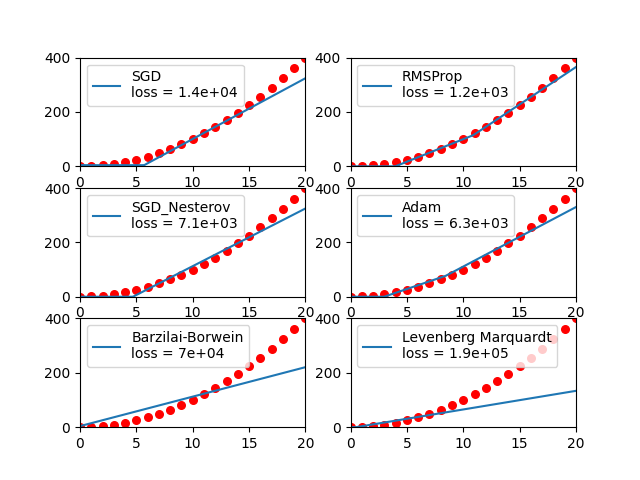
\includegraphics[scale=0.7]{Figuras/REG.png}
\caption{Resultados da aplicação dos métodos ao Problema 1 (Regressão de  $y = x^2$). Fonte: Autor} 
\label{REG}
\end{figure}


\noindent
Note que o melhor desempenho foi do \textbf{RMSProp}, método com passo adaptativo. Pode-se perceber que os 2 métodos quasi-Newton obtiveram os piores resultados no teste.


\subsection*{Comparação dos métodos no Problema 2}
Para o problema 2, foi fixada uma arquitetura de rede \textbf{30-24-30-35-1}, com 3 camadas ocultas. A inicialização dos pesos foi aleatória, porém a mesma para todos os métodos. O tamanho do lote (\textbf{batch\_size}) escolhido foi de 150 dados.
A Figura \ref{FRAUD} apresenta as curvas de Precision-Recall de cada um dos métodos, além do valor da área debaixo delas, indicado por \textit{AUC} na legenda.

\begin{figure}[H]
\center
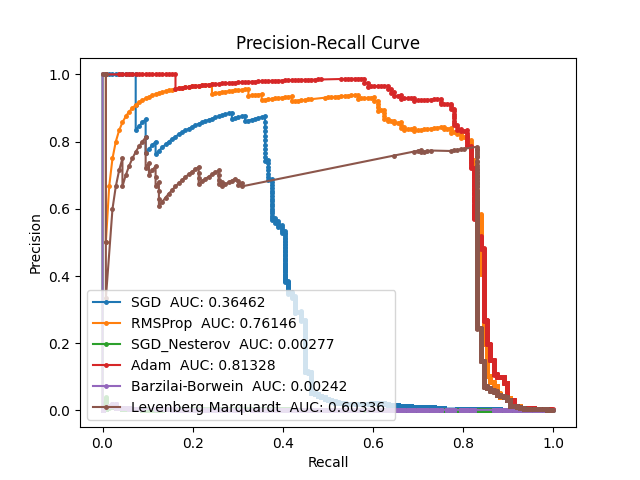
\includegraphics[scale=0.8]{Figuras/FRAUD.png}
\caption{Comparação das curvas de Precision-Recall dos métodos aplicados ao Problema 2. Fonte: Autor} 
\label{FRAUD}
\end{figure}


\noindent
O método \textbf{Adam} foi o que mais se destacou, obtendo o maior valor de AUPRC, e os métodos \textbf{SGD\_Nesterov} e \textbf{Barzilai-Borwein} tiveram um desempenho muito abaixo dos outros. Talvez com outras inicializações de parâmetros esses métodos poderiam apresentar melhorias.
As curvas de Precision-Recall são montadas variando os \textit{tresholds} de arredondamento e registrando os valores de Precision e de Recall. Foram registradas, também, as \textbf{matrizes de confusão} dos métodos para o \textit{treshold} de $0.5$. Essas matrizes estão apresentadas na Figura \ref{CONFM}.


\begin{figure}[H]
\center
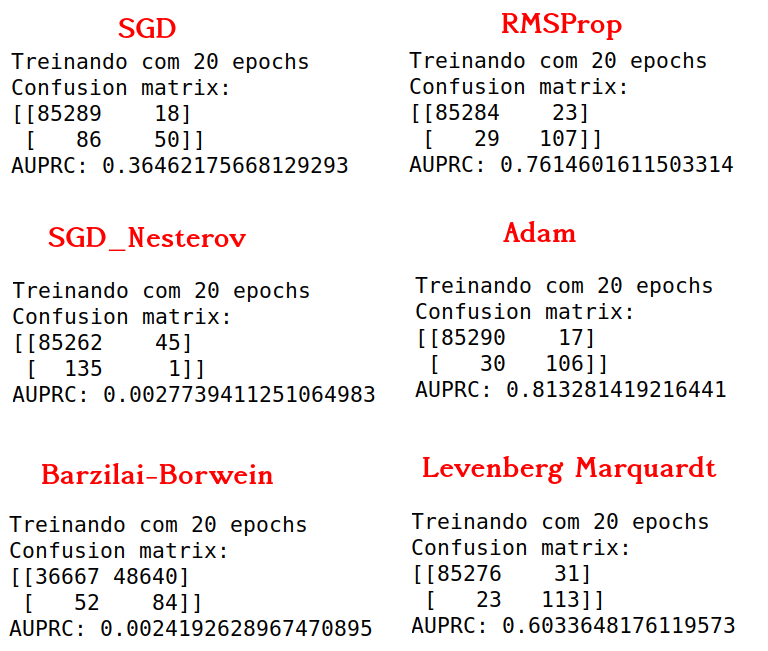
\includegraphics[scale=0.5]{Figuras/CONFMAT.png}
\caption{Comparação das matrizes de confusão dos métodos aplicados ao Problema 2. Fonte: Autor} 
\label{CONFM}
\end{figure}


\noindent
Pode-se perceber que o método com mais fraudes detectadas foi o Levenberg Marquardt, com 113 acertos, mas deixou 23 passarem e detectou indevidamente 31 transações limpas. O método RMSProp foi o segundo com mais detecções, com 107 fraudes identificadas e um desempenho mais equilibrado que o anterior. Já o método Adam foi o terceiro com mais fraudes detectadas, com 106, porém foi o mais balanceado de todos os métodos no teste. É interessante notar que a utilização da AUPRC (Área sob a curva de Precision-Recall) revela diferenças mais sutis entre os resultados de cada método do que as matrizes de confusão. Como a curva considera diversos \textit{tresholds} de arredondamento, ela realça a forma como cada método lida com o desbalanceamento do \textit{dataset}.

\subsection*{Comparação com o Keras}
Foi feita uma comparação entre o método Adam implementado no projeto e o método Adam presente na biblioteca Keras, ambos aplicados ao Problema 2. Para isso, os dados foram embaralhados da mesma maneira, a arquitetura de rede \textbf{30-24-30-35-1} aplicada ao Keras e os dados divididos como nos demais testes de deteção de fraudes. Fazendo os testes com 20 \textit{epochs} e \textit{batch\_size} 32, foram obtidos os resultados apresentados na Figura \ref{AVK}.

\begin{figure}[H]
\center
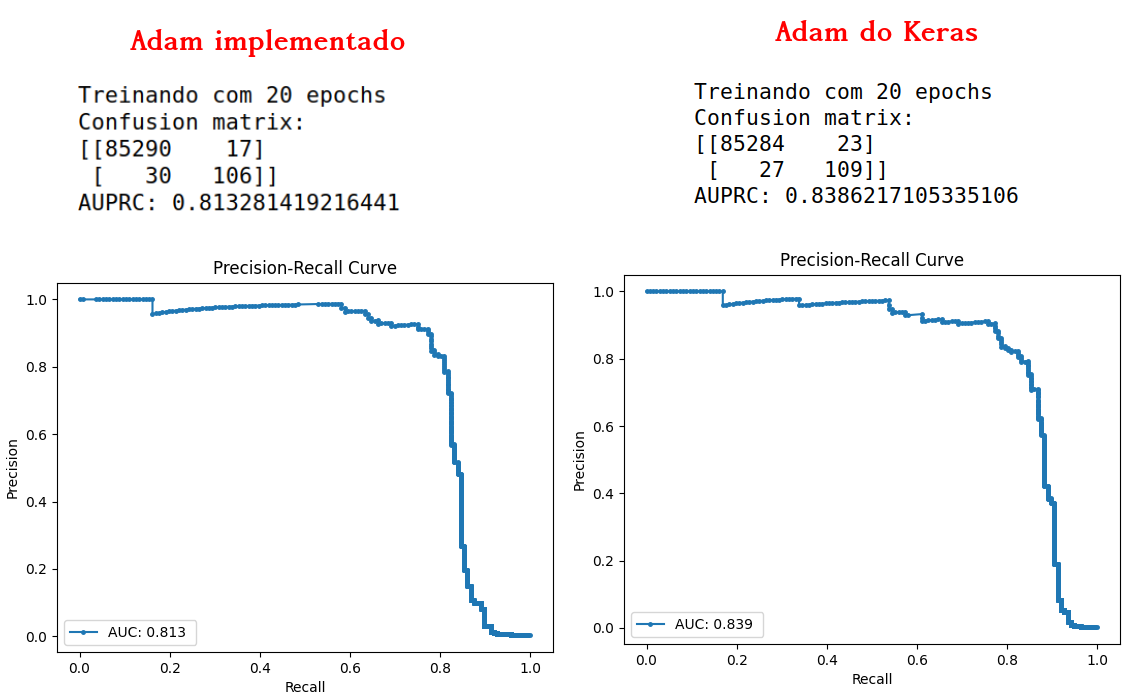
\includegraphics[scale=0.5]{Figuras/ADAM_VS_KERAS.png}
\caption{Comparação da implementação do Adam com o Adam da biblioteca Keras. Fonte: Autor} 
\label{AVK}
\end{figure}


\noindent
Observando os valores de \textbf{AUPRC}, é possivel notar que o desempenho do algoritmo implementado no presente projeto foi levemente inferior ao do método da biblioteca Keras. As matrizes de confusão apresentadas, que são para um \textit{treshold} de 0.5, demonstram que o método implementado no projeto detectou 3 fraudes a menos, porém obteve mais acertos no geral. Claramente não há garantia de que os resultados possam ser extendidos para outros pontos iniciais ou até mesmo arquiteturas de rede, mas a proximidade dos resultados aos de uma biblioteca bem estabelecida tem caráter positivo para o projeto.



\subsection*{Testes com o método de \cite{bmLS}}
\subsubsection*{Aplicado ao Problema 1, variando $\alpha$}
O primeiro teste realizado foi a aplicação do método ao Problema 1, com 3 diferentes valores de $\alpha$, o que implica em 3 níveis de exigência durante a busca linear pelo $\lambda$. Os resultados do teste estão apresentados na Figura \ref{LMBL_SQ} 
\begin{figure}[H]
\center
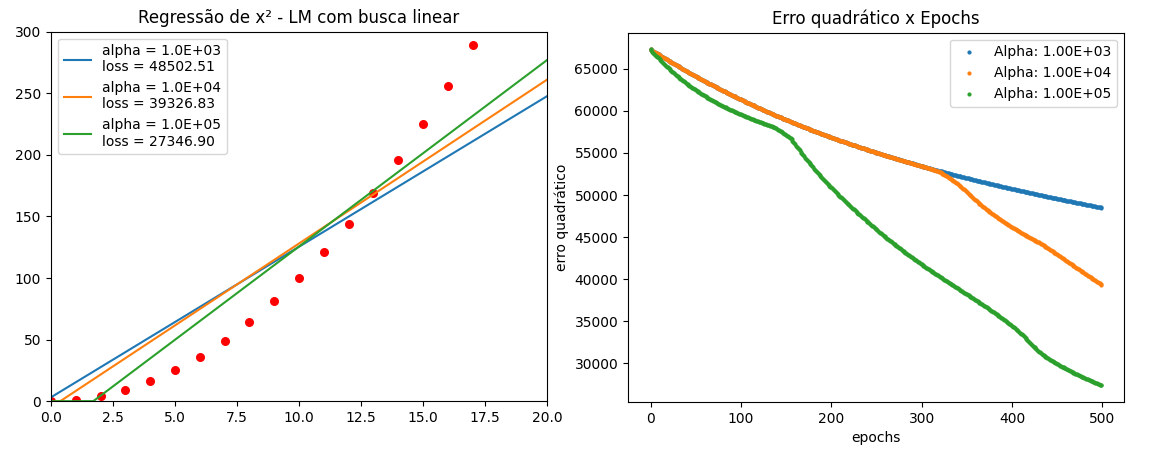
\includegraphics[scale=0.5]{Figuras/REG_lmbl.png}
\caption{Comparação de diferentes valores de $\alpha$ para o método de \cite{bmLS}. Fonte: Autor} 
\label{LMBL_SQ}
\end{figure}
Note que maiores valores de $\alpha$ implicam em um decrescimento mais rápido da função, afinal serão feitas mais buscas lineares. Entretanto, o tempo de execução não escala bem com o crescimento de $\alpha$, afinal cada vez mais iterações terão o loop de busca, como pode ser observado na Figura \ref{LMBL_time}.
\begin{figure}[H]
\center
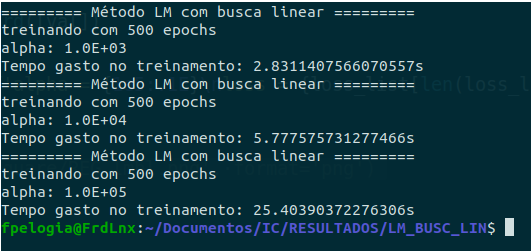
\includegraphics[scale=0.6]{Figuras/lmbl_square_t.png}
\caption{Comparação do tempo de execução com diferentes valores de $\alpha$ para o método de \cite{bmLS}. Fonte: Autor} 
\label{LMBL_time}
\end{figure}

\subsubsection*{Explorando os resultados de complexidade}
O artigo \cite{bmLS} afirma que o método atinge uma precisão $\varepsilon$ após $|log \varepsilon|$ avaliações de função quando os vetores gradiente são uniformemente linearmente independentes. Para experimentar esse resultado, foram feitos 3 testes: um dentro do caso proposto e outros 2 fora. Para esses testes, foi utilizada uma arquitetura de rede \textbf{1-2-1}, como apresentada na Figura \ref{1-2-1}, com funções de ativação $f(x) = x$.
\begin{figure}[H]
\center
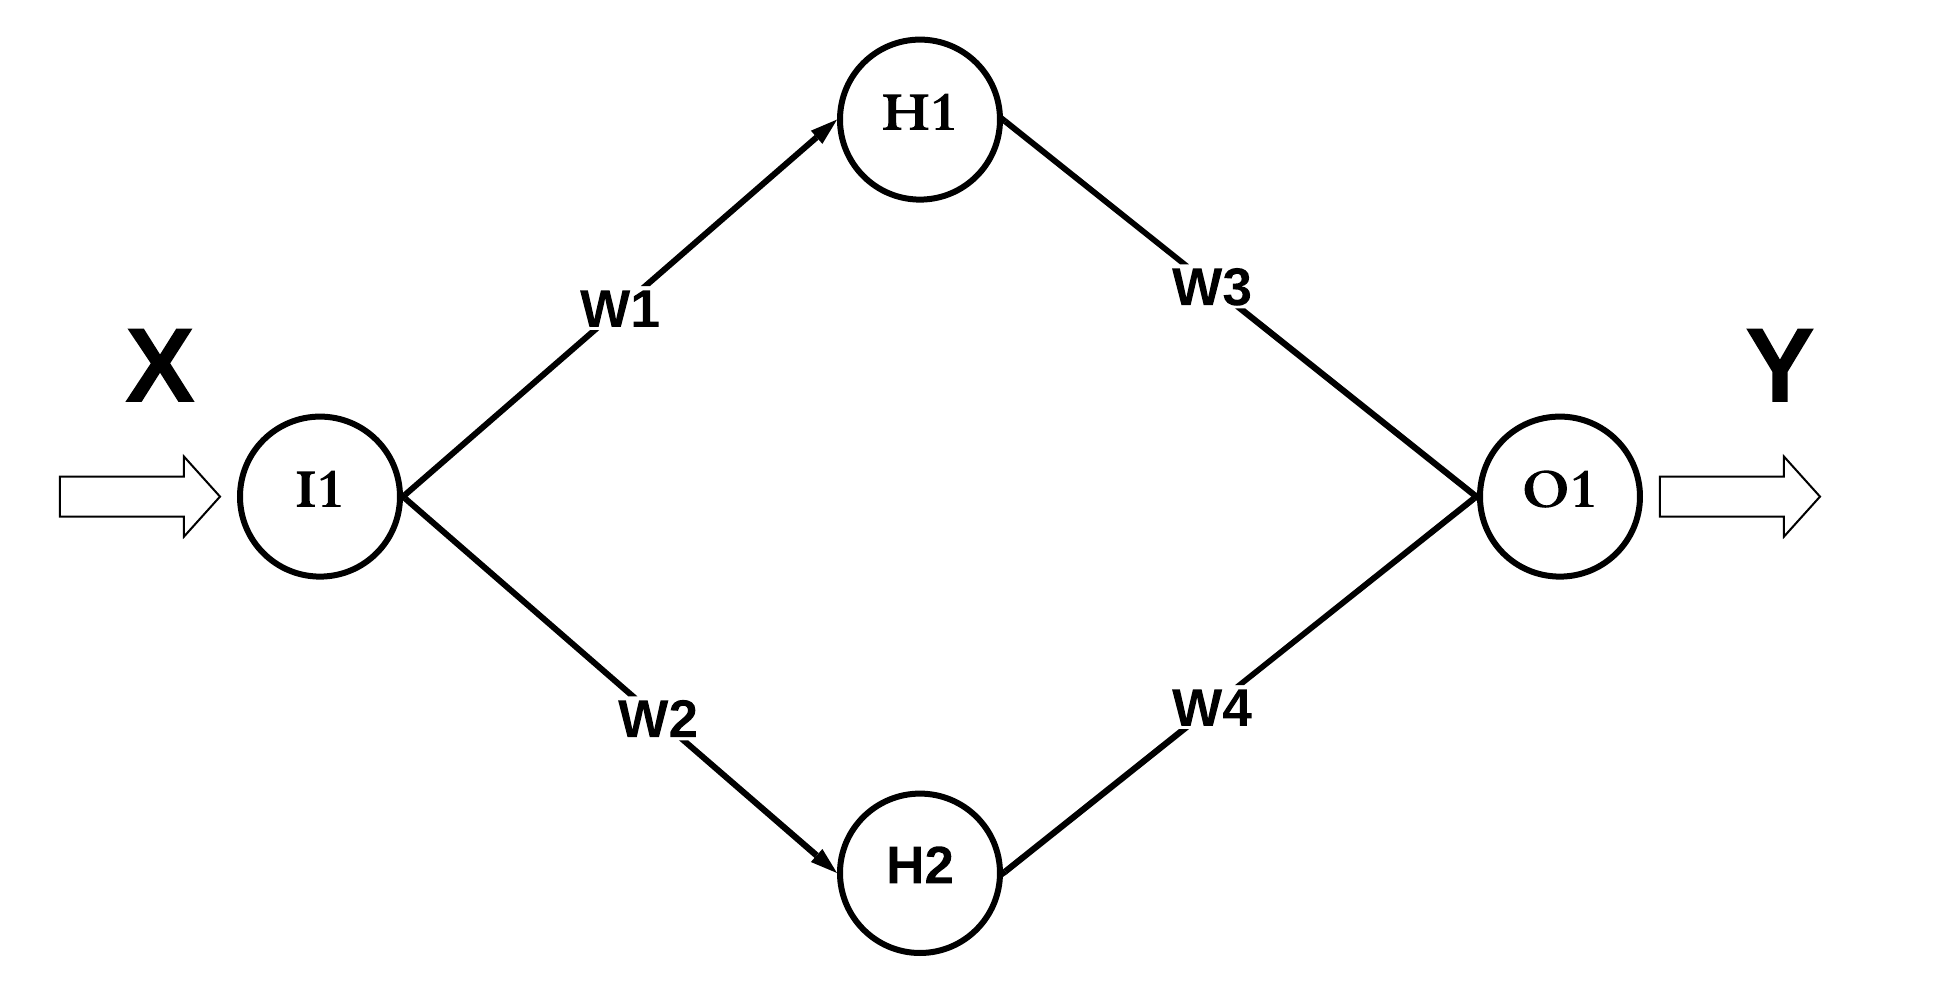
\includegraphics[scale=0.2]{Figuras/1-2-1.png}
\caption{Rede neural 1-2-1. Fonte: Autor} 
\label{1-2-1}
\end{figure}
Para esses testes, foram removidos os parâmetros \textbf{bias}, para que a predição resultasse em uma reta 
$$y = (w_1w_3 + w_2w_4)\cdot x = m\cdot x,$$
que estará sempre fixada na origem e apenas a sua inclinação é variável. A inicialização escolhida foi $$\begin{pmatrix}w_1 \\ w_2\end{pmatrix} = \begin{pmatrix}1 \\ 2\end{pmatrix} \quad \text{e} \quad \begin{pmatrix}w_3 & w_4\end{pmatrix} = \begin{pmatrix}3 & 4\end{pmatrix}.$$

Para o primeiro teste, apenas 1 dado de treinamento foi enviado: $x_1 = 1 \quad y_1 = 1^2 = 1$.
Note que, havendo apenas um dado de treinamento, existirá apenas 1 gradiente:
$$\nabla f_1(w)^T = \begin{pmatrix}-x_1 w_3 & -x_1 w_4 & -x_1 w_1 & -x_1 w_2  \end{pmatrix},$$
o que implica que não há dependências lineares, correspondendo ao caso de interesse para a afirmação do artigo.
Assim, a Figura \ref{lmbl1} apresenta o resultado da aplicação do método a esse caso, utilizando uma precisão de $1\times10^{-4}$ e $\alpha = 1\times10^{2}$.

\begin{figure}[H]
\center
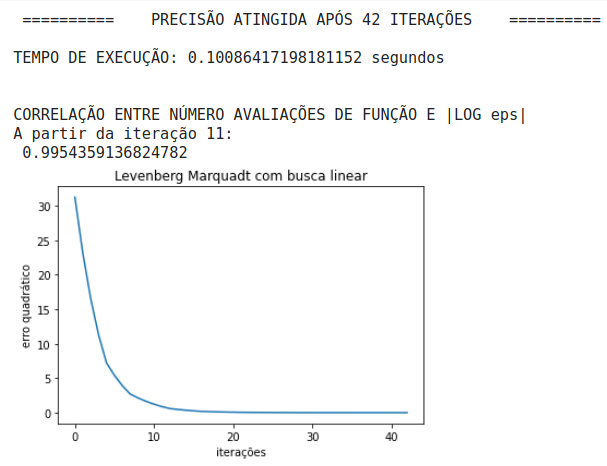
\includegraphics[scale=0.7]{Figuras/lmbl1.png}
\caption{Teste do método de \cite{bmLS} com 1 dado (gradiente LI). Fonte: Autor} 
\label{lmbl1}
\end{figure}

É possível notar que o método convergiu com facilidade e a correlação entre o número de avaliações de função e $|log \varepsilon|$ foi de aproximadamente $0.995$, sendo coerente com os resultados do artigo. A correlação foi medida a partir das iterações com erro abaixo de 1.\\

Caso sejam enviados 2 dados de treinamento, note que os gradientes serão:
$$\nabla f_1(w)^T = \begin{pmatrix}-x_1 w_3 & -x_1 w_4 & -x_1 w_1 & -x_1 w_2  \end{pmatrix}$$
$$ = x1 \cdot \begin{pmatrix}-w_3 & -w_4 & -w_1 & - w_2  \end{pmatrix},$$
$$\nabla f_2(w)^T = \begin{pmatrix}-x_2 w_3 & -x_2 w_4 & -x_2 w_1 & -x_2 w_2  \end{pmatrix},$$
$$ = x2 \cdot \begin{pmatrix}-w_3 & -w_4 & -w_1 & - w_2  \end{pmatrix},$$
Devido ao termo $\begin{pmatrix}-w_3 & -w_4 & -w_1 & - w_2  \end{pmatrix}$, os gradientes mostram-se linearmente \textbf{dependentes}.

Os 2 outros testes, seguem a ideia apresentada na Figura \ref{t23}.
\begin{figure}[H]
\center
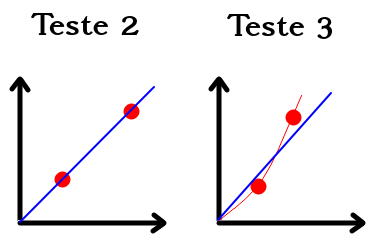
\includegraphics[scale=0.5]{Figuras/2testes.png}
\caption{Ideia dos testes 2 e 3 para o método de \cite{bmLS}. Fonte: Autor} 
\label{t23}
\end{figure}
O segundo teste envia $x = [1,1.5]$ e $y = [1,1.5]$, que é um caso em que a aproximação exata por uma reta é possível, embora os gradientes inda sejam linearmente dependentes. A Figura \ref{lmbl2} apresenta o resultado da aplicação do método a esse caso, utilizando uma precisão de $1\times10^{-4}$ e $\alpha = 1\times10^{2}$.
\begin{figure}[H]
\center
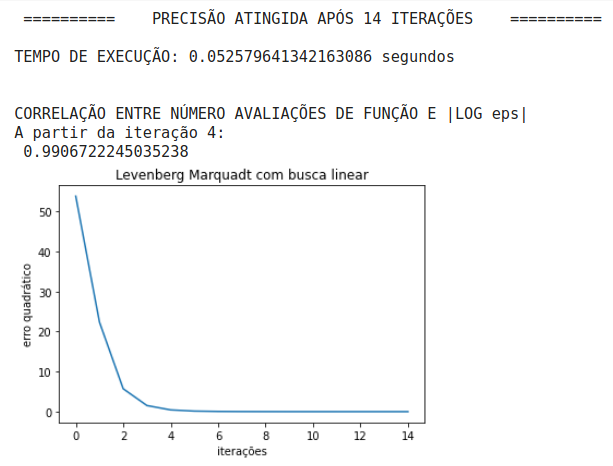
\includegraphics[scale=0.7]{Figuras/lmbl2.png}
\caption{Teste do método de \cite{bmLS} com 2 dados y = x (gradientes LD, mas aproximação possível). Fonte: Autor} 
\label{lmbl2}
\end{figure}

Embora o caso tenha gradientes linearmente dependentes, fugindo do cenário proposto pelo artigo, o caráter linear do problema permitiu uma convergência fácil, com a correlação entre o número de avaliações de função e $|log \varepsilon|$ sendo de aproximadamente $0.991$. A correlação foi medida a partir das iterações com erro abaixo de 1.


O terceiro teste envia $x = [1,1.5]$ e $y = [1,2.25]$, que é um caso em que a aproximação do modelo não conseguirá exatidão e os gradientes seguem sendo linearmente dependentes. A Figura \ref{lmbl3} apresenta o resultado da aplicação do método a esse caso, utilizando uma precisão de $1\times10^{-4}$ e $\alpha = 1\times10^{2}$. 

\begin{figure}[H]
\center
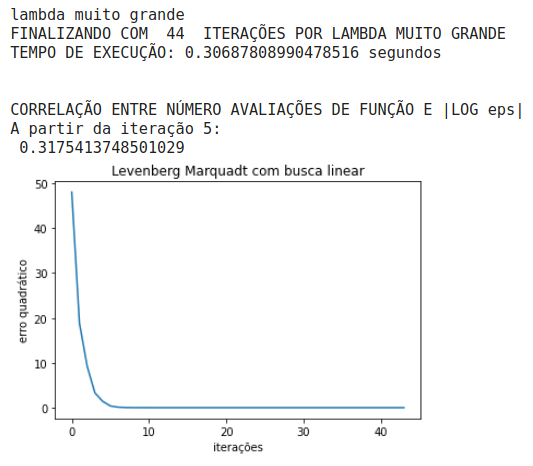
\includegraphics[scale=0.7]{Figuras/lmbl3.png}
\caption{Teste do método de \cite{bmLS} com 2 dados $y = x^2$ (gradientes LD). Fonte: Autor} 
\label{lmbl3}
\end{figure}

Note que o método teve mais dificuldade e a correlação entre o número de avaliações de função e $|log \varepsilon|$ foi de aproximadamente $0.318$. Entretanto, isso ocorre pois a função não chega a zero, mas a um valor mínimo que deveria ser levado em conta para calcular essa correlação.

Assim, para encontrar esse valor, sabemos que
$$\begin{pmatrix}1 \\ 1.5\end{pmatrix}m = \begin{pmatrix}1 \\ 2.25\end{pmatrix},$$
e, por quadrados mínimos, a melhor aproximação vem de
$$\begin{pmatrix}1 & 1.5\end{pmatrix}\begin{pmatrix}1 \\ 1.5\end{pmatrix}m = \begin{pmatrix}1 & 1.5\end{pmatrix}\begin{pmatrix}1 \\ 2.25\end{pmatrix}.$$
Assim,
$$3.25 m = 4.375,$$
o que implica que
$$m = \frac{35}{26} = 1.346153846.$$
Logo, desejamos ver o valor mínimo que $f$ assume:
$$f_{min} = \frac{1}{2}  ((1m - 1)^2 + (1.5m - 2.25)^2 ) $$
$$= \frac{9}{104} = 0.08653846154 \approx 0.0865  $$

Assim, podemos utilizar uma precisão de parada um pouco maior que esse valor e considerar $|log(\varepsilon - 0.0865)|$ para fazer a correlação. Dessa forma, o efeito gerado seria o mesmo de somar esse valor à função objetivo da minimização. Assim, a Figura \ref{a2sh} apresenta os resultados desse teste para $\alpha = 1\times 10^{2}$.

\begin{figure}[H]
\center
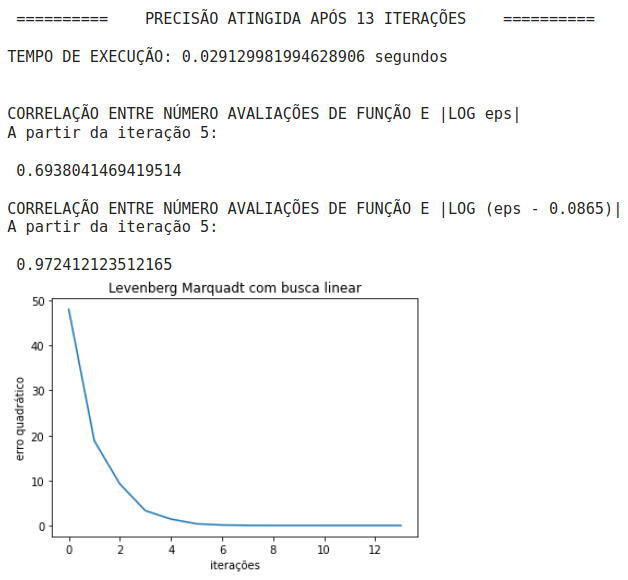
\includegraphics[scale=0.7]{Figuras/a2sh.png}
\caption{Teste com 2 dados $y = x^2$ (gradientes LD), utilizando o valor $0.0866$ como condição de parada e $\alpha = 1\times 10^{2}$. Fonte: Autor} 
\label{a2sh}
\end{figure}

Note que agora o método consegue atingir a precisão e que a correlação do número de avaliações de função com $|log(\varepsilon - 0.0865)|$ vale aproximadamente $0.972$, seguindo o resultado de complexidade do artigo, embora os gradientes sejam linearmente dependentes. 

\section{Conclusão}
Portanto, as realizações do período de vigência da bolsa foram importantes para o aprendizado do aluno, possibilitando o contato com assuntos que não seriam abordados durante sua graduação e podem ser relevantes para a vida profissional. Além disso, o aluno teve seu primeiro contato com o ambiente acadêmico e de pesquisa. O projeto proporcionou, também, uma maior familiaridade com a linguagem de programação Python e algumas de suas bibliotecas de matemática e ciência de dados.

Nos períodos referentes a ambos os relatórios, foram feitas revisões bibliográficas de artigos e a verificação prática de seus resultados em cenários levemente divergentes. A aplicação dos métodos estudados à detecção de fraudes foi importante para comparar a eficácia de cada estratégia a esse tipo de problema. Isso é relevante, pois a detecção de anomalias é largamente utilizada para diferentes domínios de aplicação na atualidade.


\newpage

\section*{Utilização de recursos da reseva técnica da bolsa}

Durante o período abordado por este relatório, não houve utilização dos recursos financeiros da reserva técnica da bolsa.

\newpage

\printbibliography

\end{document}



